% BEGIN generated cost-parts figure
% Generated by figures/cost-parts/build_figure.py; data in the same directory.
\begin{figure}[t]
\centering
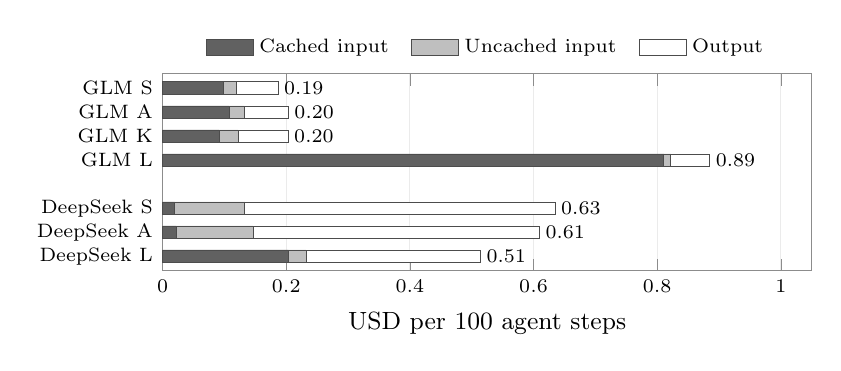
\begin{tikzpicture}
\begin{axis}[xbar stacked,scale only axis,width=0.68\columnwidth,height=2.5cm,bar width=4.6pt,
xmin=0,xmax=1.05,ymin=0.4,ymax=8.6,xtick={0,0.2,0.4,0.6,0.8,1.0},
ytick={1,2,3,5,6,7,8},yticklabels={DeepSeek L,DeepSeek A,DeepSeek S,GLM L,GLM K,GLM A,GLM S},
xlabel={USD per 100 agent steps},tick label style={font=\scriptsize},label style={font=\small},
axis line style={black!45},tick style={black!45},ytick style={draw=none},xmajorgrids,grid style={black!8},
legend style={at={(0.5,1.03)},anchor=south,legend columns=3,font=\scriptsize,draw=none,
/tikz/every even column/.append style={column sep=6pt}},legend cell align=left,clip=false]
\addplot[fill=black!62,draw=black!70,line width=0.3pt,area legend] coordinates {(0.09861,8) (0.1075,7) (0.09117,6) (0.8107,5) (0.01936,3) (0.0219,2) (0.2035,1)};
\addlegendentry{Cached input}
\addplot[fill=black!25,draw=black!70,line width=0.3pt,area legend] coordinates {(0.02032,8) (0.02463,7) (0.03086,6) (0.01135,5) (0.1137,3) (0.1243,2) (0.02842,1)};
\addlegendentry{Uncached input}
\addplot[fill=white,draw=black!70,line width=0.3pt,area legend] coordinates {(0.06789,8) (0.07137,7) (0.08104,6) (0.06314,5) (0.5019,3) (0.4634,2) (0.2824,1)};
\addlegendentry{Output}
\node[font=\scriptsize,anchor=west,inner sep=2pt] at (axis cs:0.1868,8) {0.19};
\node[font=\scriptsize,anchor=west,inner sep=2pt] at (axis cs:0.2035,7) {0.20};
\node[font=\scriptsize,anchor=west,inner sep=2pt] at (axis cs:0.2031,6) {0.20};
\node[font=\scriptsize,anchor=west,inner sep=2pt] at (axis cs:0.8851,5) {0.89};
\node[font=\scriptsize,anchor=west,inner sep=2pt] at (axis cs:0.6349,3) {0.63};
\node[font=\scriptsize,anchor=west,inner sep=2pt] at (axis cs:0.6096,2) {0.61};
\node[font=\scriptsize,anchor=west,inner sep=2pt] at (axis cs:0.5143,1) {0.51};
\end{axis}
\end{tikzpicture}
\caption{What the steps paid for: cost per 100 agent steps at the list prices of
Table~\ref{tab:prices}, split by token type and pooling each policy's agent and summarization requests
over its runs; DeepSeek's L covers the four tasks with S/A pairs.}
\label{fig:costparts}
\end{figure}
% END generated cost-parts figure
